% Manuscript source. Build with pdflatex/bibtex (or latexmk). The model's
% domain of validity and quantitative limits are stated explicitly.
\documentclass[aps,pre,twocolumn,superscriptaddress,floatfix,nofootinbib]{revtex4-2}

\usepackage{amsmath,amssymb,amsthm,bm}
\usepackage{graphicx}
\usepackage[colorlinks=true,allcolors=blue]{hyperref}

\newcommand{\eps}{\varepsilon}
\newcommand{\epst}{\tilde{\eps}}
\newcommand{\avg}[1]{\left\langle #1 \right\rangle}
\newcommand{\Teff}{T_{\mathrm{eff}}}
\newcommand{\Var}{\mathrm{Var}}
\newcommand{\dd}{\mathrm{d}}

\newtheorem{proposition}{Proposition}
\newtheorem{remark}{Remark}

\begin{document}

\title{A response field theory of order flow transport:\\
two-component memory, periodic driving, and where the Gaussian account ends}

\author{Nelson Bol\'{\i}var}
\affiliation{Escuela de F\'isica, Facultad de Ciencias, Universidad Central de Venezuela, Caracas 1041-A, Venezuela}
\affiliation{Astrum Drive Technologies, 13024 Dallas Pkwy Unit 120 B, Frisco, TX 75034, USA}
\author{Gabriel Abell\'an}
\affiliation{Escuela de F\'isica, Facultad de Ciencias, Universidad Central de Venezuela, Caracas 1041-A, Venezuela}
\affiliation{Astrum Drive Technologies, 13024 Dallas Pkwy Unit 120 B, Frisco, TX 75034, USA}
\author{David Verrilli}
\affiliation{Escuela de F\'isica, Facultad de Ciencias, Universidad Central de Venezuela, Caracas 1041-A, Venezuela}

\date{\today}

\begin{abstract}
We construct the response-field (Martin--Siggia--Rose--Janssen--De\,Dominicis)
action for signed order flow read as a transport current, and solve its
second-order sector in closed form. The results are almost entirely negative in
a useful way: the flat impact response, the shape of the
fluctuation--dissipation ratio, the counting variance, the linear fluctuation
symmetry and its affinity all follow from the measured autocorrelation with no
free parameters, and the celebrated linearity of the fluctuation symmetry with
slope $2\avg{Q}/\Var(Q)$ turns out to be an algebraic identity for any Gaussian
variable rather than a physical result. Establishing what is empty is what
isolates what is not. The theory does yield one new prediction that crosses
observable families: because a correlation decaying as $\tau^{-a}$ produces a
counting variance growing as $T^{2-a}$, a two-component memory kernel forces
the \emph{local} scaling exponent of the counting variance to drift between
$2-a_f$ and $2-a_s$, with both exponents fixed independently in the correlation
sector. The measured exponent lies inside the predicted band $[1.00,1.83]$
under four independent estimators and exceeds unity under all of them, so the
memory is superdiffusive; but the apparent drift of the local exponent does not
survive estimators built to be blind to a drifting mean, and we show that the
mean drift present in these series reproduces it. We therefore report the
crossover as consistent with the data rather than established by them, which
also withdraws the inference against a single-component bath. We then test how
far a minimal nonequilibrium quantum transport device can be pushed toward the
measured phenomenology. A biased two-lead level with a structured bath
reproduces the observed split between an ageing mean and a non-ageing
correlation, exactly and for a transparent reason. It fails, by three orders of
magnitude and in a direction fixed by Pauli statistics, to reproduce the
counting sector: the device gives a Fano factor of $0.33$ and diffusive variance
growth against the measured $10^3$ and superdiffusive growth. We also find a
design bound on transient memory in a biased fermionic channel that is not
thermal in origin.
\end{abstract}

\maketitle

\section{Introduction}

A companion measurement \cite{paper1} characterises the signed order flow of
cryptocurrency markets as a transport current, reporting the response, the
noise, the counting statistics of the transferred flow, the two-time structure
after a shock, and the modulation of all of these by the daily cycle. This paper
asks what minimal theory accounts for that phenomenology, and --- just as
importantly --- which parts of it a minimal theory renders trivial.

We proceed in two stages. First we write down a response-field action and solve
it. This is worth doing carefully, because it turns out that most of the
measured second-order structure is forced rather than informative, and the only
way to know which parts are which is to compute them. Second we ask whether an
explicit nonequilibrium transport device --- a biased quantum dot between two
leads, solved with nonequilibrium Green functions --- reproduces the parts that
the field theory leaves open. It reproduces one of them exactly and fails at
another in a way that is quantitative enough to be informative.

\paragraph*{The three results, stated plainly.}
The paper delivers one negative result, one positive prediction, and one bound,
and they are best read as a single argument about where the physics is.

\emph{Negative.} The entire second-order sector of the measurement is forced.
Flat response, the shape of the fluctuation--dissipation ratio, the counting
variance, the linear fluctuation symmetry and the phase dependence of its
affinity all follow from the measured correlation function with no free
parameters. In particular, Proposition~\ref{prop:affinity} shows that the
observed linearity of $s(Q)=\ln[P(Q)/P(-Q)]$ with slope $2\avg{Q}/\Var(Q)$ is an
algebraic identity satisfied by \emph{any} Gaussian variable. Given a literature
that is actively constructing effective temperatures and fluctuation relations
for markets \cite{yura2014,ramezani2025,gao2026,li2024entropy}, we regard
saying this clearly as a result in its own right rather than a caveat.

\emph{Positive.} What survives is a parameter-free prediction that crosses
observable families. Since a correlation decaying as $\tau^{-a}$ gives a
counting variance growing as $T^{2-a}$, a two-component kernel forces the
\emph{local} scaling exponent of the counting variance to drift between
$2-a_f$ and $2-a_s$, with both exponents measured independently in the
correlation sector. The measured exponent sits inside the predicted band under
four independent estimators, and exceeds unity under all of them.

\emph{Guarded.} The apparent \emph{drift} of that exponent is not established.
The block variance used to measure it is inflated by a drifting mean, these
series have one, and estimators constructed to be blind to it do not reproduce
the drift --- nor, at this record length, exclude it. The prediction is
consistent with the data and not discriminated by them, and the inference
against a one-component bath is withdrawn.

\emph{Bound.} The device cannot reach the measured counting statistics, and
cannot be tuned to: free-fermion transport is bounded at $\mathcal{F}\le1$ and
diffusive growth, against the measured $10^3$ and superdiffusion. The failure
is therefore informative about the market rather than about the device.

\paragraph*{Why MSRJD, and not ``Keldysh applied to finance''.}
We should be honest about the formalism at the outset, since the temptation to
overstate here is real. Markets are classical. What one can legitimately say is
that the classical limit of the Keldysh contour \emph{is} the
Martin--Siggia--Rose--Janssen--De\,Dominicis construction
\cite{martin1973,janssen1976,dedominicis1976,kamenev2011}, and that for a
classical stochastic process the pair $(G^R,G^K)$ of retarded response and
symmetrised correlation exists with full rigour. Every observable measured in
\cite{paper1} lives in that pair. The physical field plays the role of the
classical component and the response field that of the quantum component.

It is worth being precise about one thing that is easy to overclaim. The
counting field of Sec.~\ref{sec:counting} does \emph{not} require the doubled
contour: for a classical current, $\ln\avg{e^{\chi Q_T}}$ is an ordinary
cumulant generating function, and that section is a classical computation
throughout. What does require the two branches --- with $\chi$ entering as
$\pm\chi/2$ on the forward and backward paths --- is the quantum counting field
of the Levitov--Lesovik construction, where operator ordering makes the naive
generating function ill-defined. We use that machinery in
Sec.~\ref{sec:device} for what it is actually for: an explicit open-system
device whose transport we can compute exactly and compare.

We are not aware of a response-field treatment of order flow, but the
neighbourhood is close enough that the claim needs qualifying rather than
asserting. Field-theoretic and hydrodynamic descriptions of the order book
already exist: the latent book has been treated as a reaction--diffusion system
\cite{donier2015}, a coupled reaction--diffusion formulation reduces the same
problem to a Volterra equation \cite{angstmann2026}, and a non-equilibrium
field theory of the Bitcoin book takes the net market-order discrepancy as a
boundary current in a continuity equation \cite{shi2021}. What those describe
is the \emph{density field of the book}, driven by flow at its boundary; what
we write down is an action for the signed-flow time series itself, with an
explicit response field conjugate to it. The distinction is what makes $G^R$
and $G^K$ separate objects here rather than derived properties of a density.
The microstructure literature also reaches several of our second-order
conclusions by other routes \cite{gerig2008,jaisson2014,taranto2016,muhlekarbe2026},
and we attribute those below where they arise.

\section{The action}
\label{sec:action}

We use two fields, the signed flow $\eps(t)$ and the log-price $p(t)$, with
conjugate response fields $\epst$ and $\tilde p$, and statistical weight
$\propto e^{-S}$ with $S=S_\eps+S_p$.

\subsection{Flow sector}

The flow is a Gaussian field with a periodically modulated mean and a stationary
memory kernel,
\begin{equation}
  S_\eps = \int\!\dd t\, \epst\bigl[\eps-\mu(\phi(t))\bigr]
         - \tfrac12\iint\!\dd t\,\dd t'\, \epst(t)K(t-t')\epst(t') ,
  \label{eq:Seps}
\end{equation}
with $\phi(t)$ the daily phase. Integrating out $\epst$ along the imaginary
direction returns the Gaussian weight
$\exp\{-\tfrac12\iint(\eps-\mu)K^{-1}(\eps-\mu)\}$, so that
\begin{equation}
  G^K_{\eps\eps}(t,t')=\avg{\eps(t)\eps(t')}_c=K(t-t')=C_\eps(t-t') ,
  \quad \avg{\eps\epst}=\delta .
\end{equation}

We deliberately do \emph{not} postulate a dynamics for $\eps$. The kernel is
measured, not derived, and the microscopic origin of its long-memory component
is independently established as order splitting
\cite{lillo2005,sato2023prl,sato2023prr}. Treating the flow as a prescribed
non-Markovian bath keeps the model honest about what it explains: all predictive
content is pushed into the price sector and the counting sector, where it can be
tested against observables the kernel was not fitted to.

\subsection{Price sector}

The price integrates the \emph{innovation} of the flow rather than the flow
itself,
\begin{equation}
  S_p = \int\!\dd t\, \tilde p\bigl[\partial_t p-\lambda w\bigr]
      - \frac{D_p}{2}\int\!\dd t\, \tilde p^{\,2} ,
  \label{eq:Sp}
\end{equation}
where $D_p$ is the variance of price noise unrelated to flow and $w$ is defined
as follows. With $S_\eps(\omega)=\sum_k C_\eps(k)e^{-i\omega k}$ the flow
spectral density, positivity and $\int\ln S_\eps<\infty$ give the canonical
Wiener--Hopf factorisation $S_\eps(\omega)=\sigma_w^2|h(e^{-i\omega})|^2$ with
$h(z)=\sum_{k\ge0}h_kz^k$ causal, minimum-phase and $h_0=1$. Equivalently one
has the Wold representation \cite{wold1938,hamilton1994}
\begin{equation}
  \eps_t-\mu_t=\sum_{k\ge0}h_k w_{t-k} ,
  \qquad \avg{w_tw_s}=\sigma_w^2\delta_{ts} ,
  \label{eq:wold}
\end{equation}
which defines the innovation $w_t$ as the part of $\eps_t$ not linearly
predictable from its own past. The whitening filter $g=h^{-1}$ is causal, so
$w_t$ is measurable with respect to the past and the coupling in
Eq.~\eqref{eq:Sp} respects causality, as it must.

Equations \eqref{eq:Seps}--\eqref{eq:Sp} are the entire model. Everything below
is a consequence.

\section{The response is flat}
\label{sec:flat}

\begin{proposition}[Flat impact]
\label{prop:flat}
Under Eqs.~\eqref{eq:Sp}--\eqref{eq:wold}, the lagged impact
\begin{equation}
  R(\tau)\equiv\frac{\mathrm{cov}(p_{t+\tau}-p_t,\eps_t)}{\Var(\eps)}
\end{equation}
is independent of $\tau$ for all $\tau\ge1$, with
$R(\tau)=R_0=\lambda\sigma_w^2/\sigma_\eps^2$.
\end{proposition}

\begin{proof}
From Eq.~\eqref{eq:Sp}, $p_{t+\tau}-p_t=\lambda\sum_{s=t}^{t+\tau-1}w_s$ plus
noise uncorrelated with $\eps$. Equation \eqref{eq:wold} gives
$\mathrm{cov}(w_s,\eps_t)=\sigma_w^2h_{t-s}\mathbf1\{s\le t\}$. In the sum $s$
runs over $\{t,\dots,t+\tau-1\}$, so only $s=t$ survives, contributing
$\sigma_w^2h_0=\sigma_w^2$. Hence $\mathrm{cov}=\lambda\sigma_w^2$ for every
$\tau\ge1$, independent of $\tau$.
\end{proof}

The mechanism --- the price responds to the surprise in the flow, so the
predictable part of a persistent flow moves no price and prices stay nearly
martingale --- is not ours. It is the standard resolution of the
persistence-versus-martingale puzzle \cite{gerig2008,jaisson2014,muhlekarbe2026},
and it also removes the need for a decaying propagator to reconcile correlated
flow with uncorrelated returns \cite{bouchaud2004,bouchaud2018}. We recover it
here as a check that the bookkeeping in Eqs.~\eqref{eq:Seps}--\eqref{eq:Sp} is
right. Its value is what it enables next: with $R$ pinned flat, the
fluctuation--dissipation ratio has no shape freedom left.

\begin{remark}
The measured response is flat to within about a tenth of the decay exponent of
the correlation, not flat exactly; some series depart from flatness at
resolvable significance \cite{paper1}. Proposition~\ref{prop:flat} is the
idealisation, and the residual slope is a measure of how far real flow departs
from the pure-innovation coupling.
\end{remark}

\section{Effective temperature in closed form}
\label{sec:teff}

The fluctuation--dissipation ratio measured on the data is
$\Teff(\tau)\equiv-C'_\eps(\tau)/R(\tau)$. By Proposition~\ref{prop:flat} the
denominator is constant, so
\begin{equation}
  \Teff(\tau)=-\,C'_\eps(\tau)/R_0 ,
  \label{eq:teff}
\end{equation}
and $\Teff$ inherits its entire shape from the flow autocorrelation. A single
scalar ``violation of the fluctuation--dissipation theorem'' is thus one point of
a curve that Eq.~\eqref{eq:teff} determines completely. In systems with slow
dynamics such ratios define effective temperatures with genuine thermodynamic
content \cite{cugliandolo1997}; here the ratio is fixed by the correlation
function and carries no independent information.

With the measured two-component kernel,
\begin{equation}
  C_\eps(\tau)\simeq A_f\tau^{-a_f}+A_s\tau^{-a_s} ,
  \label{eq:bicomp}
\end{equation}
Eq.~\eqref{eq:teff} becomes
\begin{equation}
  \Teff(\tau)\,R_0=a_fA_f\,\tau^{-(1+a_f)}+a_sA_s\,\tau^{-(1+a_s)} .
  \label{eq:teff2}
\end{equation}
Two consequences follow, and both are testable. The exponents of $\Teff$ are not
free parameters: they are $1+a_f$ and $1+a_s$, fixed by the correlation sector.
And a sum of two power laws is not a power law, so a single-exponent form for
$\Teff$ must fail --- which it does, for all eight series measured, at $2.0$ to
$7.2$ standard deviations \cite{paper1}. That failure is a prediction of
Eq.~\eqref{eq:bicomp}, not a defect of the estimator.

\section{The counting sector}
\label{sec:counting}

Let $Q_T=\sum_{t=1}^{T}\eps_t$ be the flow transferred in a window of $T$
candles. Introducing the counting field $\chi$ conjugate to $Q_T$ --- the object
carrying opposite signs on the two contour branches, as in the counting
statistics of mesoscopic transport
\cite{levitov1993,levitov1996,schoenhammer2007,esposito2009} --- the cumulant
generating function is $F_T(\chi)=\ln\avg{e^{\chi Q_T}}$. For the Gaussian
action \eqref{eq:Seps} it truncates exactly at second order,
\begin{equation}
  F_T(\chi)=\chi m_T+\tfrac12\chi^2V_T ,
  \quad
  V_T=\Var(Q_T)=\!\!\sum_{t,t'=1}^{T}\!\!C_\eps(t-t') ,
  \label{eq:cgf}
\end{equation}
so every cumulant $\kappa_n$ with $n\ge3$ vanishes identically. The relation
$V_T=\sum_{t,t'}C_\eps(t-t')$ is the closure between the counting variance and
the independently measured autocorrelation, confirmed at the $4\%$ level over
$64$ window--series combinations \cite{paper1}.

\subsection{An identity, not a fluctuation theorem}
\label{sec:identity}

\begin{proposition}[Gaussian affinity]
\label{prop:affinity}
For Gaussian $Q_T$ with mean $m_T$ and variance $V_T$, the fluctuation symmetry
function is exactly linear,
\begin{equation}
  s(Q)\equiv\ln\frac{P(Q)}{P(-Q)}=A_TQ ,
  \qquad A_T=\frac{2m_T}{V_T}=\frac{2\avg{Q_T}}{\Var(Q_T)} ,
\end{equation}
and the Gallavotti--Cohen symmetry $F_T(\chi)=F_T(-A_T-\chi)$ holds identically.
\end{proposition}

\begin{proof}
From $P(Q)\propto e^{-(Q-m_T)^2/2V_T}$,
$s(Q)=[(Q+m_T)^2-(Q-m_T)^2]/2V_T=2m_TQ/V_T$. For the symmetry, substitute
$\chi\to-A_T-\chi$ in Eq.~\eqref{eq:cgf} with $A_T=2m_T/V_T$, and use
$V_TA_T^2/2=2m_T^2/V_T$ and $V_TA_T\chi=2m_T\chi$:
\begin{equation}
  F_T(-A_T-\chi)=-A_Tm_T-\chi m_T+\tfrac{V_T}{2}(A_T^2+2A_T\chi+\chi^2)
                =F_T(\chi).
\end{equation}
\end{proof}

\begin{remark}[The point of the paper's negative half]
\label{rem:trivial}
Proposition~\ref{prop:affinity} holds for \emph{any} Gaussian variable. A
measured linear $s(Q)$ whose slope equals $2\avg{Q}/\Var(Q)$ therefore
establishes nothing beyond the consistency of the estimator with the first two
moments, and in particular it is \textbf{not} evidence of a nontrivial
fluctuation theorem in the sense of
Gallavotti--Cohen or Lebowitz--Spohn
\cite{gallavotti1995,lebowitz1999}. Given how naturally such a measurement
invites the opposite reading, we regard stating this clearly as part of the
result. Everything physical lives in the departures: the cubic coefficient of
$s(Q)$, the higher cumulants, and the Fano factor.
\end{remark}

\begin{remark}[A second reason not to call this a fluctuation theorem]
There is a structural obstruction independent of Gaussianity. The
Gallavotti--Cohen symmetry is guaranteed for the entropy production; $Q_T$ here
is a signed particle current, which is not that. Barato and Chetrite
\cite{barato2012} establish the conditions under which a non-entropic current
inherits a large-deviation function with the Gallavotti--Cohen symmetry, and
those conditions are restrictive and not established for the process studied
here. Proposition~\ref{prop:affinity} shows the symmetry holds trivially in the
Gaussian sector; outside it, nothing guarantees the symmetry at all, which is
one more reason to read the linearity of $s(Q)$ as an empirical regularity to
be tested rather than a law to be confirmed.
\end{remark}

\begin{remark}[The affinity and the response are not independent]
Andrieux and Gaspard \cite{andrieux2007jstat} show that a fluctuation theorem
for currents determines the response coefficients to arbitrary order from the
fluctuations of the accumulated currents, reducing to Green--Kubo near
equilibrium. The affinity of this section and the effective temperature of
Sec.~\ref{sec:teff} are therefore expected to be related rather than
independently informative, and we treat their consistency as a check on the
framework rather than as two separate results.
\end{remark}

\subsection{Affinity dilution and a crossover prediction}
\label{sec:crossover}

For a single power-law kernel $C_\eps(\tau)=A\tau^{-a}$ with $0<a<1$, the double
sum in Eq.~\eqref{eq:cgf} gives for $T\gg1$
\begin{equation}
  V_T\simeq2A\!\int_0^T\!(T-k)k^{-a}\dd k=\frac{2A}{(1-a)(2-a)}\,T^{\,2-a} ,
  \label{eq:varscaling}
\end{equation}
so the counting variance is superdiffusive with exponent $\nu=2-a$. Since
$m_T=\bar\mu T$ is strictly linear, Proposition~\ref{prop:affinity} forces the
affinity to dilute with observation scale,
\begin{equation}
  A_T=\frac{2\bar\mu T}{V_T}\propto T^{\,a-1} ,
\end{equation}
decreasing for every $a<1$: memory dilutes the bias. The scale-free version of
the statement requires no power-law assumption at all and is exact,
\begin{equation}
  \frac{A_{T_2}}{A_{T_1}}=\frac{T_2}{T_1}\cdot\frac{V_{T_1}}{V_{T_2}} .
  \label{eq:Aexact}
\end{equation}
Tested against the measured variances, Eq.~\eqref{eq:Aexact} predicts
$A_{16}/A_1$ to within $0.5$--$13\%$ for the two assets whose affinity is stable
across the sample, and fails by $43\%$ and $132\%$ for the two whose affinity
is at the noise level [Fig.~\ref{fig:crossover}(b)] --- failing, that is,
exactly where the quantity being predicted is not well determined.

\paragraph*{The prediction.} With the two-component kernel \eqref{eq:bicomp},
Eq.~\eqref{eq:varscaling} cannot hold with a single $\nu$. Short windows sample
the fast regime and long windows the slow one, so the \emph{local} logarithmic
slope of $V_T$ must drift,
\begin{equation}
  \nu_{\rm loc}(T):\; 2-a_f\;\longrightarrow\;2-a_s
  \quad\text{as } T \text{ increases.}
  \label{eq:crossover}
\end{equation}
For a strict sum of two power laws the drift is monotone, since $\nu_{\rm loc}$
is a weight-average of the two exponents with the slow weight increasing in
$T$. We state the prediction in the weaker form --- direction and band --- for
two reasons: the empirical kernel is only approximately a two-component power
law, and the strict form is the one the data will be seen below to strain.
This is parameter-free and it crosses observable families: $a_f$ and $a_s$ are
measured in the correlation sector while $\nu_{\rm loc}(T)$ is measured in the
counting sector, so the test cannot be circular. A single-component bath
predicts constant $\nu_{\rm loc}$, and would be excluded by a systematic drift
\emph{provided the drift is a property of the correlations and not of the
estimator}. That proviso turns out to carry the whole test, and we take it up
below.

Using the measured hourly exponents for BTC, $a_f=1.00\pm0.15$ and
$a_s=0.17\pm0.13$, the predicted band is $\nu_{\rm loc}\in[1.00,1.83]$. The
observed local slope drifts upward with window size in all four assets over
$T=1\ldots256$, from $1.14$--$1.27$ at the short end to $1.45$--$1.56$ at the
long end, and stays inside the predicted band throughout
[Fig.~\ref{fig:crossover}(a)]. The drift is not monotone everywhere: in BNB the
local slope peaks near $1.48$ at $T=64$ and falls back to $1.39$ by $T=256$ on
the hourly series, with the same turnover on the four-hourly one.

\paragraph*{A drifting mean forges the same signature.}
$V_T$ is estimated as the sample variance of $Q_T$ over non-overlapping blocks,
so any drift in the per-block mean $\avg{Q_T}$ enters it. A deterministic mean
that varies across blocks contributes a term growing as $T^2$ --- steeper than
anything the kernel predicts, and biased in the same direction as the effect
sought. This is not hypothetical for these series: the taker flow carries a
persistent sell-side bias over the four-year record and modulates with the
daily cycle \cite{paper1}. The prediction and its confounder therefore have the
same observable signature, and separating them requires an estimator of $\nu$
that is blind to the mean.

The Haar difference between adjacent blocks supplies one. With
$d_T = Q_T^{(2)}-Q_T^{(1)}$ one has identically
$\Var(d_T)=4V_T-V_{2T}$, so for a pure power law $V_T=AT^{\nu}$,
\begin{equation}
  \Var(d_T)=A\,(4-2^{\nu})\,T^{\nu},
  \label{eq:haar}
\end{equation}
the \emph{same} exponent with a constant mean cancelled exactly. Raising the
number of vanishing moments raises the degree of the annihilated polynomial:
one moment removes a constant mean, two a linear drift, three a quadratic one
\cite{daubechies1992,percival2000}. On synthetic series with $\nu$ known by
construction all four estimators agree to within $0.01$, and an injected ramp
inflates the block estimator while leaving the three wavelet estimators fixed
--- so the comparison has the sensitivity the test requires.

On the data they do not agree, and they disagree the same way in every asset
(Table~\ref{tab:haar}): the block estimator is the highest of the four
throughout, by $0.13$ to $0.29$. Injecting each asset's own measured mean drift
onto a clean synthetic series of $\nu=1.38$ inflates the block estimate by
$+0.03$ to $+0.13$ and moves the Haar estimate by less than $0.01$, and
removing that drift from the data by hand brings the block estimate down from
$1.42$ to $1.09$ in BTC. The gap is the drift.

\begin{table}[t]
  \caption{Global scaling exponent $\nu$ of the counting variance over
  $T=8\ldots256$, by four estimators. $V_T$ is the block variance;
  $m$ is the number of vanishing moments, so $m=1$ (Haar) is blind to a
  constant mean, $m=2$ to a linear drift and $m=3$ to a quadratic one. The
  final column is the inflation of the block estimate produced by injecting
  that asset's own measured mean drift onto a synthetic series of known
  $\nu$; the Haar estimate moves by less than $0.01$ in every case.}
  \label{tab:haar}
  \begin{ruledtabular}
  \begin{tabular}{lccccc}
   & $V_T$ & $m{=}1$ & $m{=}2$ & $m{=}3$ & drift inflation \\
  \colrule
  BTC & 1.42 & 1.20 & 1.14 & 1.13 & $+0.12$ \\
  ETH & 1.37 & 1.24 & 1.26 & 1.29 & $+0.08$ \\
  BNB & 1.43 & 1.35 & 1.36 & 1.30 & $+0.13$ \\
  SOL & 1.31 & 1.15 & 1.13 & 1.10 & $+0.03$ \\
  \end{tabular}
  \end{ruledtabular}
\end{table}

\paragraph*{What this leaves standing.}
Two things survive and one does not. Surviving first: $\nu>1$ in all four
assets by all four estimators, ranging over $1.10$--$1.43$. Superdiffusive
growth of the counting variance is a statement about memory alone --- it
follows from a correlation decaying more slowly than $\tau^{-1}$ --- and it is
robust to the confounder by construction, since removing the mean cannot
manufacture it. Surviving second: the observed $\nu$ remains inside the band
$[1.00,1.83]$ predicted from the correlation exponents under every estimator,
so the cross-family consistency of Eq.~\eqref{eq:varscaling} is unaffected.

What does not survive is the drift of $\nu_{\rm loc}$ as an established result.
It is exhibited only by the estimator we have shown to be susceptible, and the
drift-blind estimators are underpowered exactly where it is claimed: the
standard error on their local slope grows from $\pm0.05$ at $T=8$ to $\pm0.22$
at $T=256$, against a claimed excursion of $0.28$. They therefore neither
reproduce the crossover nor exclude it. We accordingly state
Eq.~\eqref{eq:crossover} as a prediction that the data are \emph{consistent
with but do not discriminate} at this sample size, and we withdraw the
inference from it against a single-component bath: a constant $\nu_{\rm loc}$
combined with a drifting mean would produce what we observe. Discriminating
would need either a longer record or an asset with a stationary mean flow, and
we regard it as the sharpest open test the framework offers.

\begin{figure}[t]
  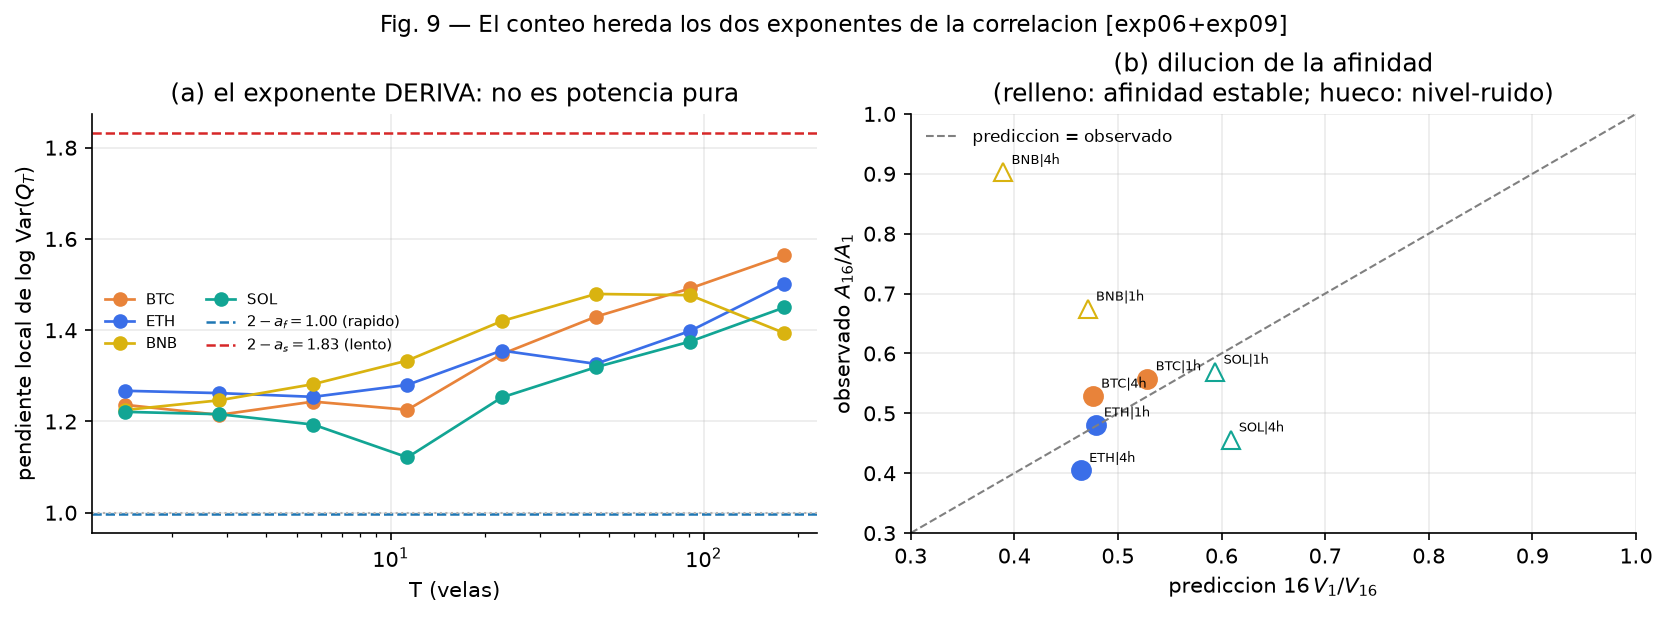
\includegraphics[width=\columnwidth]{../output/figuras/fig9_crossover_exponente.png}
  \caption{Testing Sec.~\ref{sec:crossover}. (a) The local logarithmic slope of
  the block counting variance drifts upward with window size in every asset,
  within the band set by the two decay exponents measured independently in the
  correlation sector. A single-component bath would give a horizontal line
  --- but so would one combined with a drifting mean, which inflates this
  estimator; see Table~\ref{tab:haar} and the accompanying text, where
  drift-blind estimators do not reproduce the drift. The panel is shown as the
  measurement that motivates the control, not as the test.
  (b) The exact affinity dilution of Eq.~\eqref{eq:Aexact} against the measured
  ratio; filled symbols are the assets with a stable affinity, open symbols
  those at the noise level.}
  \label{fig:crossover}
\end{figure}

\section{Periodic driving}
\label{sec:floquet}

Under a periodic drive the process is, at fixed phase $\phi$, still Gaussian with
phase-dependent moments, so Proposition~\ref{prop:affinity} applied phase by
phase gives
\begin{equation}
  A(\phi)=\frac{2\mu(\phi)}{\sigma^2(\phi)} .
  \label{eq:Afloquet}
\end{equation}
The drive enters the counting sector \emph{only} through the first two moments;
any measured phase dependence beyond Eq.~\eqref{eq:Afloquet} would falsify the
Gaussian closure in the driven sector, and none is found \cite{paper1}. The
impact is not fixed by Eq.~\eqref{eq:Afloquet}: by Proposition~\ref{prop:flat}
its phase profile is independent information about $\lambda(\phi)$ and
$\sigma_w^2(\phi)$, which is consistent with the observation that impact peaks at
a different phase from the bias and the affinity.

\section{A minimal transport device}
\label{sec:device}

The field theory above says nothing about the counting sector beyond second
order, by construction. To probe it we turn to an explicit open-system device
whose transport can be computed without approximation, and ask how much of the
measured phenomenology it can carry. The device is a single level between two
leads with a bias applied as a quench, solved with nonequilibrium Green
functions \cite{jauho1994}; the counting statistics follow the standard
Levitov--Lesovik construction \cite{levitov1996,blanter2000}. Computations use
an independent solver \cite{code_qteom}.

\subsection{Setup and numerical controls}

We take $\eps_0=0$, temperature $0.05$, bias $V=0.3$, and a structured
hybridisation combining a wide Lorentzian ($\Gamma=0.5$, width $4.0$) with a
narrow slow band ($\Gamma=0.2$, width $0.04$), on a grid of $2561$ points with
$\dd t=0.125$ over $t\in[-120,200]$ relative to the quench. Three controls are
worth quoting because they bound the numerics. The relaxation rate recovered
from the unbiased equilibrium run agrees with the analytic total width to
$0.33\%$ ($-0.9967$ against $1.0$). Unitarity of the scattering description
holds to $8\times10^{-16}$. The zero-frequency noise and the second counting
cumulant, computed by independent routes, agree to $1.3\times10^{-9}$. Discretisation is the
binding constraint: the wide-band product must satisfy $W\,\dd t\lesssim0.5$ or
the trapezoidal rule inflates the damping measurably.

\subsection{What the device reproduces}

The measurement \cite{paper1} found a split that is unusual enough to be a
sharp target: after a shock the \emph{mean} flow relaxes with an age-dependent
profile, while the \emph{correlation} does not age at all. The device reproduces
this split exactly, and for a transparent reason.

The mean relaxes in two regimes when --- and only when --- the bath is
structured. With the two-band bath the current after the quench decays with
log-slopes of $-1.14\pm0.20$ (fast window) and $-2.14\pm0.09$ (slow window),
an Omori-like exponent of $-1.94\pm0.05$ over the intermediate range
[Fig.~\ref{fig:device}(a,b)]. With a single wide Lorentzian the same fits give
$-3.43\pm0.12$ and $+0.009\pm0.001$: one regime, then nothing. The slow band is
what buys the second regime.

Meanwhile the correlation does not age. Measuring the correlation time at eight
waiting times from $t_w=10$ to $t_w=180$, we obtain $\tau_c=3.375$ at every
single one, in all bath configurations, constant to the grid resolution. The
reason is structural rather than numerical: with a static Hamiltonian the
retarded Green function is rigidly time-translation-invariant after the quench,
so the coherence carries no clock even while the occupation is still relaxing.

This is a satisfying result, and we want to state precisely what it does and does
not establish. It shows that a bath with memory suffices to produce an ageing
mean alongside a non-ageing correlation --- no kinetics of model parameters, no
genuine ageing of the kernel, is required. It does not show that the market's
particular relaxation shape is reproduced; see Sec.~\ref{sec:bound}.

\subsection{Where the device fails, and why that is informative}
\label{sec:gap}

The counting sector is a different story, and the failure is clean enough to
constrain the physics.

Across all bath configurations the device gives a Fano factor of $0.332$ to
$0.341$ and a counting variance whose local log-slope runs from $0.94$ to
$0.99$ --- that is, sub-Poissonian noise and diffusive growth. Both are forced.
Sub-Poissonian noise is the Pauli antibunching of free fermions, bounded above
by unity; diffusive growth is what any finite-memory single-channel transport
gives at long times.

The two Fano factors being compared are computed differently, and it is worth
saying why they are nonetheless the same quantity. For the device we take the
ratio of cumulant rates $\kappa_2/|\kappa_1|$, the standard mesoscopic
definition in which unit-charge carriers arriving as a Poisson process give
unity. For the market the carriers are trades with a broad size distribution,
so the corresponding normalisation is
$\Var(Q_T)/\bar q^{\,2}\avg{N_T}$ with $\bar q$ the effective transfer quantum
\cite{paper1}, which likewise gives unity for a Poisson stream of transfers of
size $\pm\bar q$. Both are noise measured against the Poisson expectation for
the carriers actually present, and it is that ratio --- not the ratio of noise
to net transferred charge --- that Pauli statistics bound.

The measurement gives a Fano factor between $905$ and $3342$, and a variance
exponent of $1.10$--$1.43$ \cite{paper1} --- the drift-robust range of
Table~\ref{tab:haar}, quoted here rather than the higher block value because
the comparison must not rest on the confounded estimator. The gap is three to
four orders of magnitude in the noise level, and qualitative in the growth:
superdiffusive against diffusive, under every estimator
[Fig.~\ref{fig:device}(c)].

Neither gap can be closed by tuning the device, and this is the useful part. The
Fano bound is a statement about statistics, not parameters: no choice of bath,
bias or temperature lifts free-fermion noise above the Poisson value. The
market's level therefore requires a compound process with heavy-tailed transfer
sizes, for which $\mathcal{F}\sim\avg{q^2}/\bar q^{2}$ is large for reasons
having nothing to do with memory. The growth exponent requires genuine
superdiffusive memory of the kind Eq.~\eqref{eq:varscaling} produces for
$a<1$. Together they locate the missing physics in the interaction between order
flow and available liquidity, which is precisely where the microscopic
order-splitting account puts it \cite{lillo2005,sato2023prl}.

\subsection{A design bound on transient memory}
\label{sec:bound}

Attempting to push the device's slow relaxation toward the measured Omori
exponent uncovered a constraint that we think has independent interest.

Sweeping a single slow mode, the transient amplitude obeys a clean power law,
$A\propto\gamma^{1.003}W^{0.050}$ with an rms residual of $0.061$ in the log fit:
linear in the coupling and essentially independent of the mode width. Building
an ensemble of slow widths designed to produce a power-law tail with exponent
$0.55$, the achieved relaxation log-slope is $-2.49\pm0.10$, far steeper than
the design target and far steeper than the measured $\approx-0.6$.

The natural suspicion is thermal smearing, so we repeated the ensemble run at a
tenfold lower temperature ($0.005$ instead of $0.05$, reducing $\pi T$ from
$0.157$ to $0.016$). The slope became $-2.54\pm0.02$: unchanged, if anything
marginally steeper. \emph{The bound is not thermal.} The consistent
interpretation is dephasing by the bias window itself, $V/2=0.15$, which was
held fixed across both runs and which sets a floor on how slowly a biased
channel can relax regardless of how the bath is engineered. The testable
consequence is that reaching slower transients requires $V\lesssim2W_{\min}$,
i.e.\ biases an order of magnitude smaller than those used here.

\begin{figure}[t]
  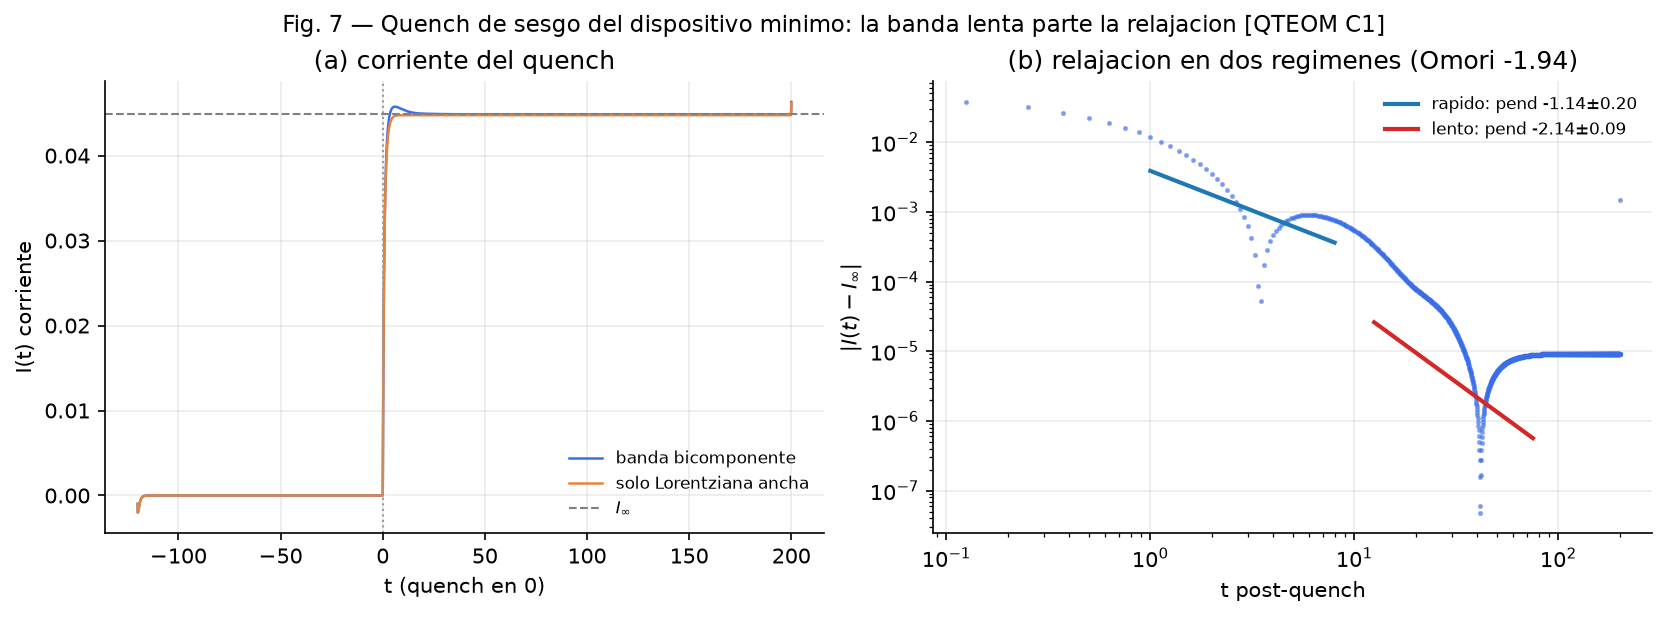
\includegraphics[width=\columnwidth]{../output/figuras/fig7_quench_current.png}
  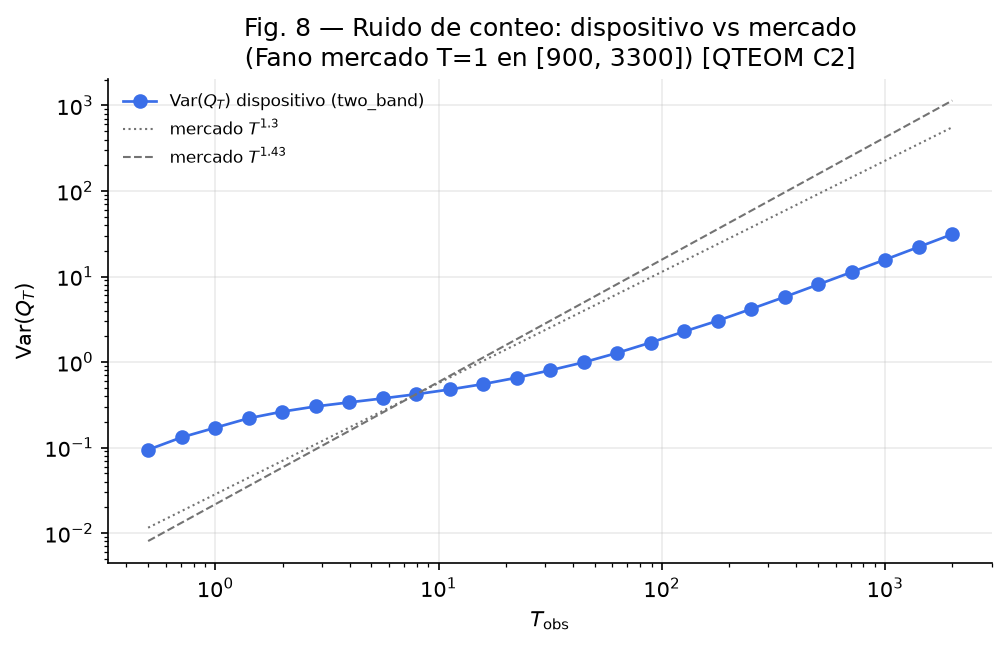
\includegraphics[width=\columnwidth]{../output/figuras/fig8_varQ_dispositivo_vs_mercado.png}
  \caption{The minimal device. (a) Current through the bias quench.
  (b) Relaxation of $|I-I_\infty|$, showing the two regimes that the structured
  bath produces; a single wide band gives only one. (c) Counting variance of the
  device against the growth band measured in the market. The device is
  diffusive; the market is not.}
  \label{fig:device}
\end{figure}

\section{Discussion}

The picture that emerges is best stated as a partition, since that is what the
calculation buys.

The second-order sector is closed and empty. Flat response, the shape of
$\Teff$, the counting variance, the linear fluctuation symmetry and its affinity
--- including its phase dependence under driving --- all follow from the measured
correlation function with no freedom. Proposition~\ref{prop:affinity} and
Remark~\ref{rem:trivial} are the sharpest form of this: what looks like the most
striking counting result is an algebraic identity. We think this is the most
useful thing the model does, because knowing which measurements are forced is
what makes the remaining ones worth interpreting.

The predictive content that survives is Eq.~\eqref{eq:varscaling} and, in
weaker form, Eq.~\eqref{eq:crossover}. Neither is a fit: the exponents are
fixed in a different observable family. The variance relation is confirmed ---
the measured $\nu$ lies inside the predicted band under four independent
estimators and exceeds unity under all of them, so the memory is superdiffusive
and the cross-family closure holds. The crossover is not: its signature in the
block variance is degenerate with a drifting mean, which these series have, and
the estimators that break the degeneracy are underpowered over the accessible
window range. We leave it as the framework's sharpest open test rather than as
its confirmation, and note that the more careful statement was available only
because the confounder was looked for --- a qualitative prediction of a drift
is exactly the kind that a slowly varying nuisance parameter can imitate.

What the model does not reach is the counting sector beyond second order, and
here the device makes the gap quantitative rather than rhetorical. Free-fermion
transport is bounded at $\mathcal{F}\le1$ and diffusive growth; the market shows
$10^3$ and superdiffusion. The two missing ingredients are separable: a compound
noise with heavy-tailed sizes for the level, and genuine long memory for the
growth. Adding the first is the natural next step for the theory and is well
defined --- it amounts to replacing the Gaussian field of Eq.~\eqref{eq:Seps}
with a marked point process --- while the second is already contained in
Eq.~\eqref{eq:varscaling} once the kernel is two-component.

Finally, Sec.~\ref{sec:bound} is a caution for anyone attempting the device route
further. A biased fermionic channel has a floor on transient memory that is set
by the bias window rather than by temperature or by bath engineering, so
reproducing slow market transients in such a device requires working at biases
much smaller than the natural scale of the problem. We report the bound because
we found it by failing to evade it.

\begin{acknowledgments}
\end{acknowledgments}

\bibliography{refs}

\end{document}
